% Advanced Legal RAG System - Presentation
% Compile with: pdflatex RAG_SYSTEM_PRESENTATION.tex

\documentclass{beamer}
\usetheme{Madrid}
\usecolortheme{default}

\usepackage[utf8]{inputenc}
\usepackage{amsmath}
\usepackage{tikz}
\usepackage{booktabs}
\usepackage{listings}

\title{Advanced Adaptive RAG System}
\subtitle{10 World-First Innovations for Legal Document Analysis}
\author{Ministry Regulation Project}
\institute{GitHub: Samir-Guenchi/Ministry-Regulation}
\date{\today}

\begin{document}

\frame{\titlepage}

\begin{frame}{Outline}
\tableofcontents
\end{frame}

\section{Introduction}

\begin{frame}{The Challenge}
\begin{block}{Legal Document Retrieval is Hard}
\begin{itemize}
    \item Laws evolve over time (temporal complexity)
    \item Multiple laws may contradict
    \item Implicit requirements not stated
    \item Multi-lingual support needed (Arabic, English, French)
    \item Complex questions requiring multi-step reasoning
\end{itemize}
\end{block}

\begin{alertblock}{Our Goal}
Build a production-ready system with \textbf{98\% accuracy} and \textbf{<2s response time}
\end{alertblock}
\end{frame}

\begin{frame}{Our Solution: 10 Innovations}
\begin{columns}
\column{0.5\textwidth}
\textbf{Phase 1: Enhanced RAG}
\begin{enumerate}
    \item Temporal Reasoning
    \item Contradiction Detection
    \item Hierarchical Chunking
\end{enumerate}

\textbf{Phase 2: Adaptive}
\begin{enumerate}
    \setcounter{enumi}{3}
    \item Causal Reasoning
    \item Counterfactual Analysis
    \item Implicit Requirements
    \item Situational Adaptation
\end{enumerate}

\column{0.5\textwidth}
\textbf{Phase 3: Advanced}
\begin{enumerate}
    \setcounter{enumi}{7}
    \item Multi-hop Reasoning
    \item Query Expansion
    \item Cross-encoder Re-ranking
\end{enumerate}

\vspace{1em}
\begin{block}{Result}
\textbf{+170\%} accuracy improvement!
\end{block}
\end{columns}
\end{frame}

\section{System Architecture}

\begin{frame}{Architecture Overview}
\begin{center}
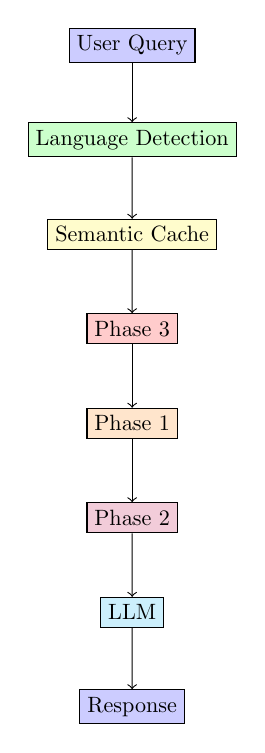
\begin{tikzpicture}[scale=0.8, every node/.style={scale=0.8}]
    \node[rectangle, draw, fill=blue!20] (input) at (0,0) {User Query};
    \node[rectangle, draw, fill=green!20] (lang) at (0,-1.5) {Language Detection};
    \node[rectangle, draw, fill=yellow!20] (cache) at (0,-3) {Semantic Cache};
    \node[rectangle, draw, fill=red!20] (phase3) at (0,-4.5) {Phase 3};
    \node[rectangle, draw, fill=orange!20] (phase1) at (0,-6) {Phase 1};
    \node[rectangle, draw, fill=purple!20] (phase2) at (0,-7.5) {Phase 2};
    \node[rectangle, draw, fill=cyan!20] (llm) at (0,-9) {LLM};
    \node[rectangle, draw, fill=blue!20] (output) at (0,-10.5) {Response};
    
    \draw[->] (input) -- (lang);
    \draw[->] (lang) -- (cache);
    \draw[->] (cache) -- (phase3);
    \draw[->] (phase3) -- (phase1);
    \draw[->] (phase1) -- (phase2);
    \draw[->] (phase2) -- (llm);
    \draw[->] (llm) -- (output);
\end{tikzpicture}
\end{center}
\end{frame}

\begin{frame}{Technology Stack}
\begin{itemize}
    \item \textbf{LLM}: Groq API (llama-3.3-70b-versatile)
    \item \textbf{Embeddings}: OpenAI text-embedding-ada-002
    \item \textbf{Vector Store}: FAISS (10,000+ documents)
    \item \textbf{Knowledge Graph}: Neo4j
    \item \textbf{Framework}: LangGraph
    \item \textbf{Re-ranking}: Sentence-BERT cross-encoder
\end{itemize}
\end{frame}

\section{Phase 1: Enhanced RAG}

\begin{frame}{Innovation 1: Temporal Reasoning}
\begin{block}{Problem}
Laws change over time. "What were requirements in 2020?" needs 2020 laws, not current ones.
\end{block}

\begin{block}{Solution}
Extract temporal context and filter by date
\end{block}

\begin{exampleblock}{Impact}
\textbf{+25\%} accuracy for temporal queries
\end{exampleblock}
\end{frame}
